\section{System Design}

In this section, we present the design of Lever. Lever is 
API-compatible with Spark Streaming, providing the mitigation transparency and
developer transparency. Considering the main objective is to minimize latency,
Lever is designed to be lightweight and to be able to make agile scheduling
decisions. We begin with an overview of the system architecture, followed by
further system details.

\subsection{System Overview}

Figure 4 overviews the architecture of Lever. Lever periodically collects and
analyzes the historical job profiles of the recurring micro-batch jobs.
Based on such information, Lever pre-schedules the data through three main
steps, i.e. identify potential stragglers, evaluate node capacity and choose
suitable helpers. Firstly, comparing each node's task finish time in the previous
batch, Lever can determine the initial state of each node. Lever also
estimates the changes of the input data rate. With these two pieces of
information, Lever estimate the state transition to predict which nodes will
behave as stragglers in next batch (for Challenge 1). Secondly, based on the fact that
micro-batch processing jobs are repetitive and periodic, Lever adopt the
Iterative Learning Control (ILC \cite{Arimoto}) model, which is designed for
tracking control of systems that work in a repetitive mode, to estimate
node capabilities (for Challenge 2). Finally, 
% considering that Lever does not have
% the accurate overview of the resource utilization during pre-scheduling, 
Lever have two strategies for choosing helpers, i.e. choosing all the nodes or
the two least loaded nodes. Lever can adaptively switch between these two
strategies to achieve high performance (for Challenge 3).

We show the timing of Lever's actions in Figure~\ref{Fig. 5:}, where we differentiate
pre-scheduling and post-scheduling techniques. It can
be seen that the post-scheduling techniques, such as Dolly, Wrangler, Speculation and SkewTune, take actions
during task processing, which would inevitably increase the task processing
latency. On the contrary,  Lever takes its action before task scheduling. As
shown in Figure~\ref{Fig. 5:}, Lever collects the needed information of the
previous micro-batches execution during batch interval between $t_1$ and $t_2$.
Then, during $t_2$ and $t_3$, Lever dispatches the input data based on the prior
pre-scheduling plan, then the tasks would be scheduled according to data
locality. In this way, Lever does not occupy any task processing time and would
not incur any data movement.  

% When come to batch $t_3$ to $t_4$, Lever schedules tasks
% according to data locality as usual. We detail each step of Lever in the
% following.
  \begin{figure*}[htbp]
    \centering
    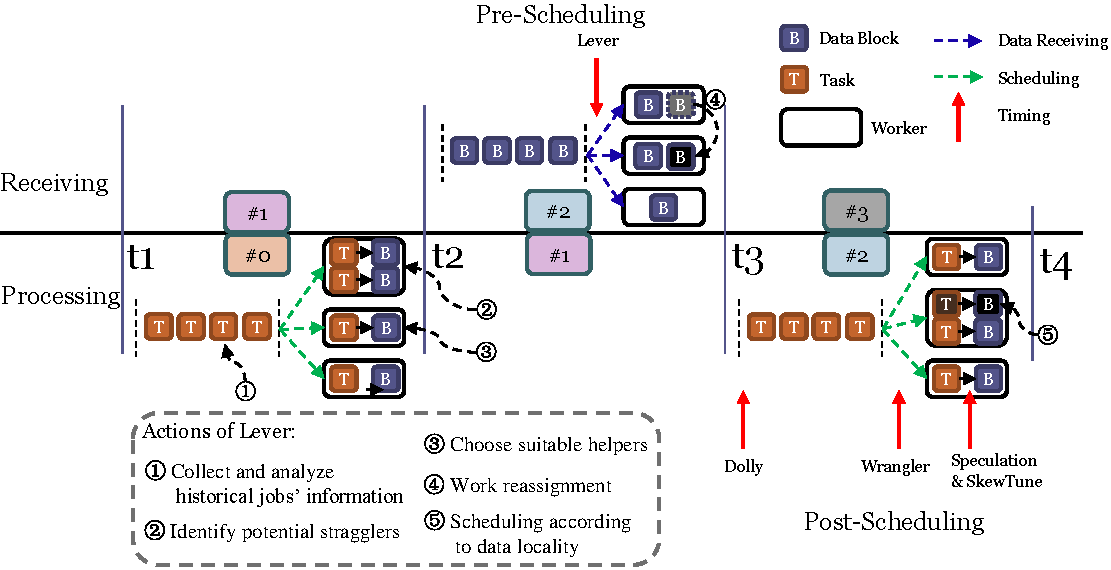
\includegraphics[width=0.8\textwidth]{FigureAction}
    \caption{Actions of Lever}
    \label{Fig. 5:}
  \end{figure*}

\subsection{Identify Potential Stragglers}

Lever predicts stragglers in the next batch according to the historical information
of the recurring jobs as well as the load fluctuation of each node. The first
step is to determine the initial stragglers. When the tasks of the last batch are
completed, Lever collects and analyze the statistics of the task execution
in each node. The node $i$'s finish time ($NFT_i$) is defined as the time from
job submission to when the last task is completed in this node.  Then, Lever sorts node
list according to $NFT_i$ in the descending order. By following the experiences
in previous work \cite{Dean2004}, we classify nodes into three
categories according to the locations of the node list. Nodes before in the
first quartile are put into the \emph{straggler group}, while those after the third 
quartile are in the \emph{faster group}. The remaining nodes are categorized as
the \emph{median group}.

The classification identifies the stragglers in the last batch. However, 
as data streaming rates vary over time and load can change across different
batches,  the state of each node may change between two consecutive batches.
Therefore, we should carefully derive the possible state transitions to
accurately identify the stragglers as follows.  First, Lever calculates the
median finish time of the \emph{straggler group}, \emph{median group} and
\emph{faster group} respectively. We denoted these values by \emph{FTOS}, \emph{FTOM},
\emph{FTOF} respectively. Second, Lever uses two degradation ratio \emph{FTM} and
\emph{MTS}. \emph{FTM} is defined as \emph{FTOM}/\emph{FTOF}, which means that 
for node $i$ in the \emph{faster group}, if $NFT_i$ 
has increased by FTM, it will be moved
from the \emph{faster group} to the \emph{median group} and vice versa.
Similarly, \emph{MTS} is defined as \emph{FTOS}/\emph{FTOM}, which means that
for node $i$ in the \emph{median group}, if $NFT_i$ has increased by MTS, it will be moved
from the \emph{median group} to the \emph{straggler group} and vice versa. We
summarize node state transition in Fig. 6.  

\begin{figure}[htbp] \centering 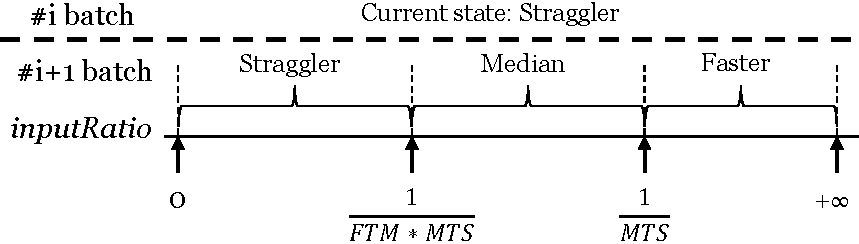
\includegraphics[width=0.42\textwidth]{FigureI2}
  \caption{An example for node state transition} \label{Fig. 6:}
\end{figure}

Based on the transition graph in Figure \ref{Fig. 6:}, in the third step, Lever
takes the load fluctuation observed on each node to predict state transition and
identify stragglers. Due to the load fluctuation, it is possible that some stragglers
in the last batch may receive less data and hence become faster in the current
batch. Similarly, the
faster nodes may possibly become stragglers in current batch. We 
use \emph{inputRatio}, defined as the ratio between the new input data rate of
current batch and the old one of the last batch, to evaluate the changes of
stream load. According to the transition graph, we define the transition rules
listed in Table~\ref{Table1}. By applying these rules, Lever finally identifies the state of
each node for the current batch.
  \begin{table}[htbp]
    \footnotesize
    \centering
    \caption{Transition rules for identifying stragglers}
    \begin{threeparttable}
    \centering
      \begin{tabular}{|p{1.5cm}|p{4.3cm}|p{1.4cm}|}
        \hline
        Initial State & Transition Conditions(inputRatio) & Final State \\
        \hline
        \multirow{3}{2cm}{Straggler} &
        (1/MTS,$+\infty$) & Straggler \\
        \cline{2-3}
        & [1/(FTM*MTS),1/MTS] & Median \\
        \cline{2-3}
        & (0,1/(FTM*MTS)) & Faster \\
        \hline
        \multirow{3}{2cm}{Median} &
        (MTS,$+\infty$) & Straggler \\
        \cline{2-3}
        & [1/FTM,MTS] & Median \\
        \cline{2-3}
        & (0,1/FTM) & Faster \\
        \hline
        \multirow{3}{2cm}{Faster} &
        (FTM*MTS,$+\infty$) & Straggler \\
        \cline{2-3}
        & [FTM,FTM*MTS] & Median \\
        \cline{2-3}
        & (0,FTM) & Faster \\
        \hline
      \end{tabular}
    \end{threeparttable}
    \label{Table1}
  \end{table}

\subsection{Computing Capacity Estimation}

After predicting the state of each node according to the input data
characteristics, we next estimate computing capacity of each node before we can
conduct pre-scheduling.

\subsubsection{Computing Capacity}


The computing capacity of a node refers to the amount of data that the node can
process in one batch. 
% As shown in Section \uppercase\expandafter{\romannumeral2}-C, recurring
% batched stream jobs have stable data properties. By analyzing the previous
% execution, We can assess these metrics exactly in the subsequent execution.
Consider the periodicity of the recurrring micro-batch jobs, we estimate
the computing capacity node based on the Iterative
Learning Control (ILC \cite{Arimoto}) model, which is designed to perform tracking control
of systems that work in a repetitive mode. Repetition allows the system to
improve the tracking accuracy through iterations. This learning process
uses information from previous repetitions to improve the estimation and can
achieve more accurate results iteratively. This scenario
is similar to the batch stream processing jobs.  

\begin{figure}[htbp] \centering
  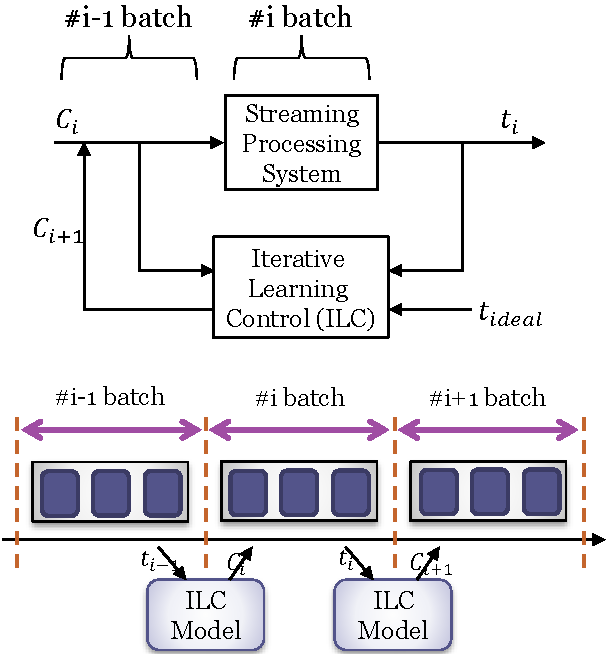
\includegraphics[width=0.36\textwidth]{FigureILC} \caption{The principle of
  evaluating computing capacity with ILC.} \label{Fig. 7:} \end{figure}

Figure \ref{Fig. 7:} shows the principle of the ILC algorithm. Our objective
is to continuously approximate the real computing capacity. The task finish
time of each node and computing capacity in the previous batch are passed to the ILC
model as the learning parameters. The ILC model is used to estimate the
computing capacity of the processing nodes for the next batch. These actions
repeat from one batch to the next. A model of estimating the capacity of a
node is of the following form:
  \begin{equation}
  C_{i+1} = C_i + K*\Delta t
  \end{equation}
   \begin{equation}
  \Delta t = t_{ideal} - t_{i}
  \end{equation}
where $C_i$ is the capacity to the stream processing system during the
$i$th batch, $\Delta t$ is the deviation between the node's finish time and the ideal
finish time during the $i$th batch. $K$ is a design parameter representing
the operations on $\Delta t$. In Lever, $K$ is set to $C_i/t_i$. $t_{ideal}$ is the
ideal finish time of the node in the $i$th batch and can be obtained by computing the
median node's finish time. We repeat this process for every batch.

\subsubsection{Theoretical Data Assignment}

In the ideal case, all the tasks should be completed simultaneously. So, the system
should increase the amount of load in the faster nodes and reduce those in
the stragglers to minimize the makespan. Assume that there are $n$ nodes. Let
\emph{$L_i$} and \emph{$C_i$} denote the input load and the computing capacity
of the $i$th node respectively. Let \emph{$L_i^\prime$} denote the input load
under Lever's pre-scheduling plan. Let $t_i$ denotes the finish time of $i$th node. We have:
  \begin{equation}
  t_i = L_i\prime / C_i
  \end{equation}
  \begin{equation}
  \sum_{i=1}^n L_i = \sum_{i=1}^n L_i\prime
  \end{equation}
In the ideal case, our optimization goal is $\delta^{2}=D(t_i)=0$. So, we have
$t_1=t_2=...=t_n$. Then, we can get
$L_1\prime/C_1=L_2\prime/C_2=...=L_n\prime/C_n$. The load \emph{$L_i^\prime$}
can be estimated  as:
  \begin{equation}
  L_i\prime =  \frac{\sum_{i=1}^n L_i}{\sum_{i=1}^n C_i}*C_i
  \end{equation}
Therefore, the load we need to migrate can be calculated as:
  \begin{equation}
  \Delta L = L_i\prime - L_i = \frac{\sum_{i=1}^n L_i}{\sum_{i=1}^n C_i}*C_i - L_i
  \end{equation}

\subsection{Choose Suitable Helpers and Reassign Work}

After grouping the nodes into three groups, we can identify that the nodes in
the faster group are eligible to act as helpers to run part of the stragglers' workload.
Nodes in the straggler group are helpees to whom helpers should provide
assistance. We distinguish two situations that Lever would face. The first one
is that there are only a small number of stragglers and fasters, while the
second one is that there are many stragglers and many fasters. The overhead of
data partitioning and task scheduling differ in these two situations. To this
end, we propose two helper choosing strategies and an adaptive method that can
adaptively choose one of them according to the actual situation.

\subsubsection{Strategies for Choosing Helpers}

\textbf{All Strategy.} With this strategy, for each straggler, all the nodes in
the faster group are selected as candidate helpers. 
% According to Section
% \uppercase\expandafter{\romannumeral3}-C, we can obtain the relatively ideal
% load distribution by the proportion of node's capacity. 
Figure~\ref{Fig. 8:} shows the
principle of the All strategy. Assume that we have $k$ helpers, the node $i$ is
characterized by the vector (\emph{$C_i$},\emph{$L_i$}). For each straggler,
characterized by (\emph{$C_s$},\emph{$L_s$}), its input data is
assigned to all the selected helpers according to their capacity and load.
The load share \emph{{$L_{sToj}$}} which is dispatched to the $j$th helper can be
denoted as:
  \begin{equation}
  L_{sToj} = \frac{L_s + \sum_{i=1}^k L_i}{C_s + \sum_{i=1}^k C_i}*C_j - L_j
  \end{equation}

This strategy is suitable for the situation that there are few stragglers and
fasters. However, if there are a large number of stragglers and fasters, the
overhead of partition and migration is significant.
  \begin{figure}[htbp]
    \centering
    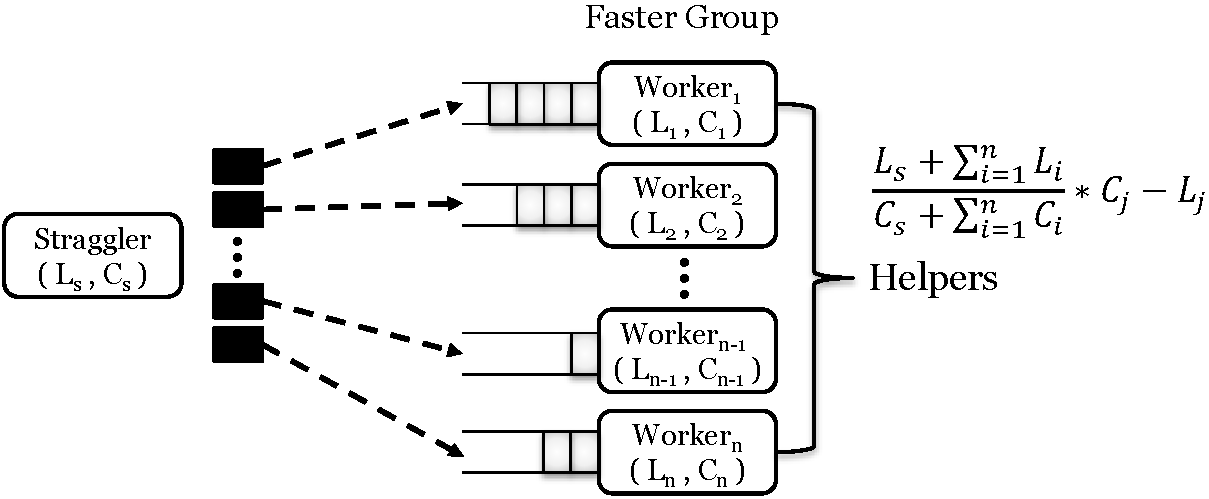
\includegraphics[width=0.48\textwidth]{FigureS1}
    \caption{The All Strategy selects all the nodes in the faster group as helpers.}
    \label{Fig. 8:}
  \end{figure}

\textbf{Two-Choice Strategy.} Based on
the-power-of-two-choice principle~\cite{Mitzenmacher1996}, the Two-Choice strategy
chooses two nodes in the faster group as the helpers for each . This strategy tries to find
two nodes, which have large computing capacity and at the same time have less
input data load, as helpers.  Figure \ref{Fig. 9:} shows the ides of the
Two-Choice strategy. First, Lever sorts the node
list according to the value \emph{$C_i$}/\emph{$L_i$} of each node in the descending order.
Then, Lever chooses the first two nodes as helpers and computes the load share for
each helper. Assume that the two selected helpers are $(C_1, L_1)$ and $(C_2,
L_2)$, and the straggler is characterized as (\emph{$C_s$},\emph{$L_s$}). The load
share \emph{{$L_{sToj}$}} which is dispatched to the $j$th helper can be denoted as:
  \begin{equation}
  L_{sToj} = \frac{L_s + L_1 + L_2}{C_s + C_1 + C_2}*C_j - L_j
  \end{equation}
After the reassignment, Lever updates each node's $C_i$ and $L_i$.
  \begin{figure}[htbp]
    \centering
    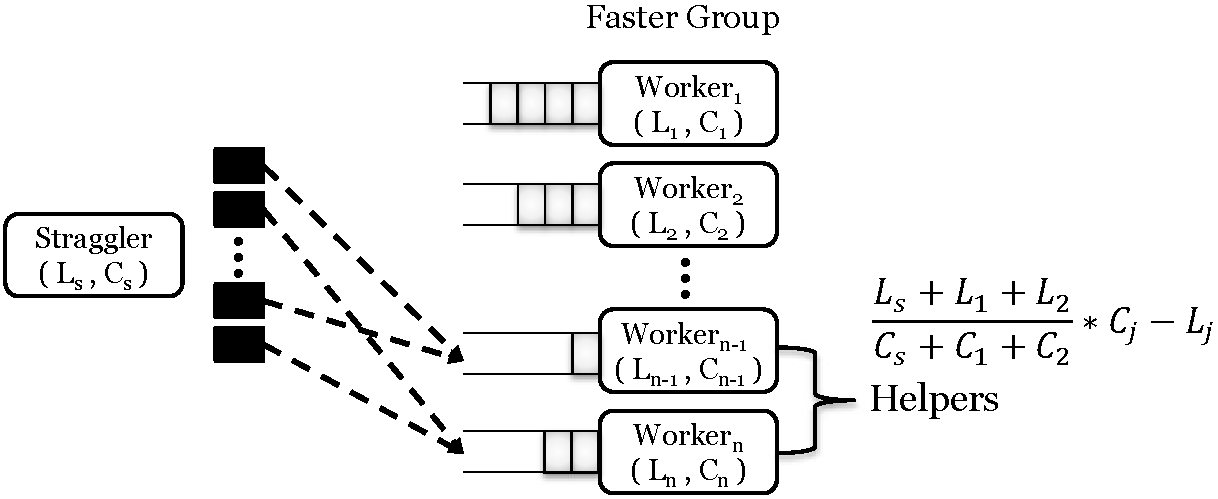
\includegraphics[width=0.48\textwidth]{FigureS2}
    \caption{Two Choice Strategy selects two nodes in faster group as helpers.}
    \label{Fig. 9:}
  \end{figure}

\subsubsection{Adaptive Helper Choosing}

The above two strategies can be used in different situations. Lever can
adaptively choose one of two strategies according to cluster's current state.
Obviously, when there are few stragglers, All is better than 
Two-Choice, because we can pre-schedule the input data as evenly as
possible.  However, if there are a large number of stragglers and fasters,
Two-Choice will behavior better, because of it can avoid the high cost of data
partition and migration. For example, if we have $s$ stragglers and $k$ fasters, this
strategy produces $s*k$ data pieces and also $s*k$ socket connections. The large
amount of $s*k$ data pieces can incur network congestion and impact the running
tasks. 

Lever takes into account the changes of latency and the value of
\#stragglers$\times$\#fasters to
make choices amount these two strategies adaptively. If \#stragglers$\times$\#fasters is larger than a threshold
value, Lever would use the Two-Choice Strategy. In addition, if
we detect that the latency of Lever is increasing with the All strategy,
we will switch to Two-Choice. The complete pseudo code of the pre-scheduling
algorithm is presented in Algorithm 1.
  \begin{algorithm}[htbp]
  \small
  \caption{Pre-Scheduling Algorithm}
  \label{Alg:1}
  \begin{algorithmic}[1]
  \STATE \textbf{Procedure} \textbf{Identify Potential Stragglers}
  \STATE \quad Get the previous batches' job execution information
  \STATE \quad Sort the nodes descending by their finish time
  \STATE \quad Group the nodes into three groups(straggler, median, faster)
  \STATE \quad Compute the input load's gradient
  \STATE \quad Transform nodes' state according to transition rules
  \STATE \quad Output final stragglers and fasters
  \STATE \textbf{End Procedure}
  \STATE \textbf{Procedure} \textbf{Evaluate Computational Capability}
  \STATE \quad In $i$th batch, compute the capacity for $i+1$th batch 
  \STATE \quad $C_{i+1} = C_i + C_i/t_i*(t_{ideal}-t_i)$
  \STATE \quad Assign the corresponding load when receiving $i+1$th data batch
  \STATE \quad In the $i+1$th batch, compute the capacity for the next batch
  \STATE \quad $C_{i+2} = C_{i+1} + \frac{C_{i+1}}{t_{i+1}}*(t_{ideal}-t_{i+1})$
  \STATE \textbf{End Procedure}
  \STATE \textbf{Procedure} \textbf{Choose Suitable Helpers and Reassign Work}
  \IF{(\#stragglers$\times$\#fasters$<$$\rho$) or (the last batch uses the All Strategy \&\& latency decreases)}
  \STATE $/*$ continue to adopt the All strategy $*/$
  \STATE Choose all the nodes as helpers
  \STATE Compute the sums of the helpers' capacities and loads respectively
  \STATE $sumOfCapa=\sum_{i=1}^n C_i$ and $sumOfLoad=\sum_{i=1}^n L_i$
  \FOR{each straggler node}
  \FOR{each helper node}
  \STATE Compute the allocated load share
  \STATE $L_{stoi}=\frac{L_s + sumOfLoad}{C_s + sumOfCapa}\times C_i-L_i$
  \STATE Update each node's $(C_i,L_i)$
  \ENDFOR
  \ENDFOR
  \ELSE
  \STATE $/*$ adopt the Two-Choice Strategy $*/$
  \STATE Sort the nodes' list according to each node's $\frac{C_i}{L_i}$ in descending order
  \STATE Choose the first two nodes as helpers
  \STATE Compute the sums of the helpers' capacities and loads respectively
  \STATE $sumOfCapa = C_1 + C_2$ and $sumOfLoad = L_1 + L_2$
  \FOR{each straggler node}
  \FOR{each helper node}
  \STATE Compute the allocated load share
  \STATE $L_{stoi}=\frac{L_s + sumOfLoad}{C_s + sumOfCapa}\times C_i-L_i$
  \STATE Update each node's $(C_i,L_i)$
  \ENDFOR
  \ENDFOR
  \ENDIF
  \STATE \textbf{End Procedure}
  \end{algorithmic}
  \end{algorithm}
